\newcommand{\overtitle}{Results}
\section{Results}

\begin{frame}
	\frametitle{\overtitle}
	\begin{itemize}
		\item Needs some fancy plots here
	\end{itemize}
\end{frame}

\begin{frame}
	\frametitle{\overtitle}
	\framesubtitle{Sample Output}
	\begin{centering}
	\texttt{%
		0 0 0 0 0 0 0 0 0 1 0 0 0 0 \\
		0 0 0 0 0 0 0 0 0 1 0 0 0 0 \\
		0 0 0 0 0 0 0 0 0 1 0 0 0 0 \\
		0 0 0 0 0 0 0 0 0 1 0 0 0 0 \\
		0 0 0 0 0 0 0 0 0 1 0 0 0 0 \\
		0 0 0 0 0 0 0 0 0 1 0 0 0 0 \\
		0 0 0 0 0 0 0 0 0 1 0 0 0 0 \\
		0 0 0 0 0 0 0 0 0 1 0 0 0 0 \\
		0 0 0 0 0 0 0 0 0 1 0 0 0 0 \\
		0 0 0 0 0 0 0 0 0 1 0 0 0 0 \\
		...
		}
	\end{centering}
\end{frame}

\begin{frame}
	\frametitle{\overtitle}
	\framesubtitle{Confusion Matrix}
	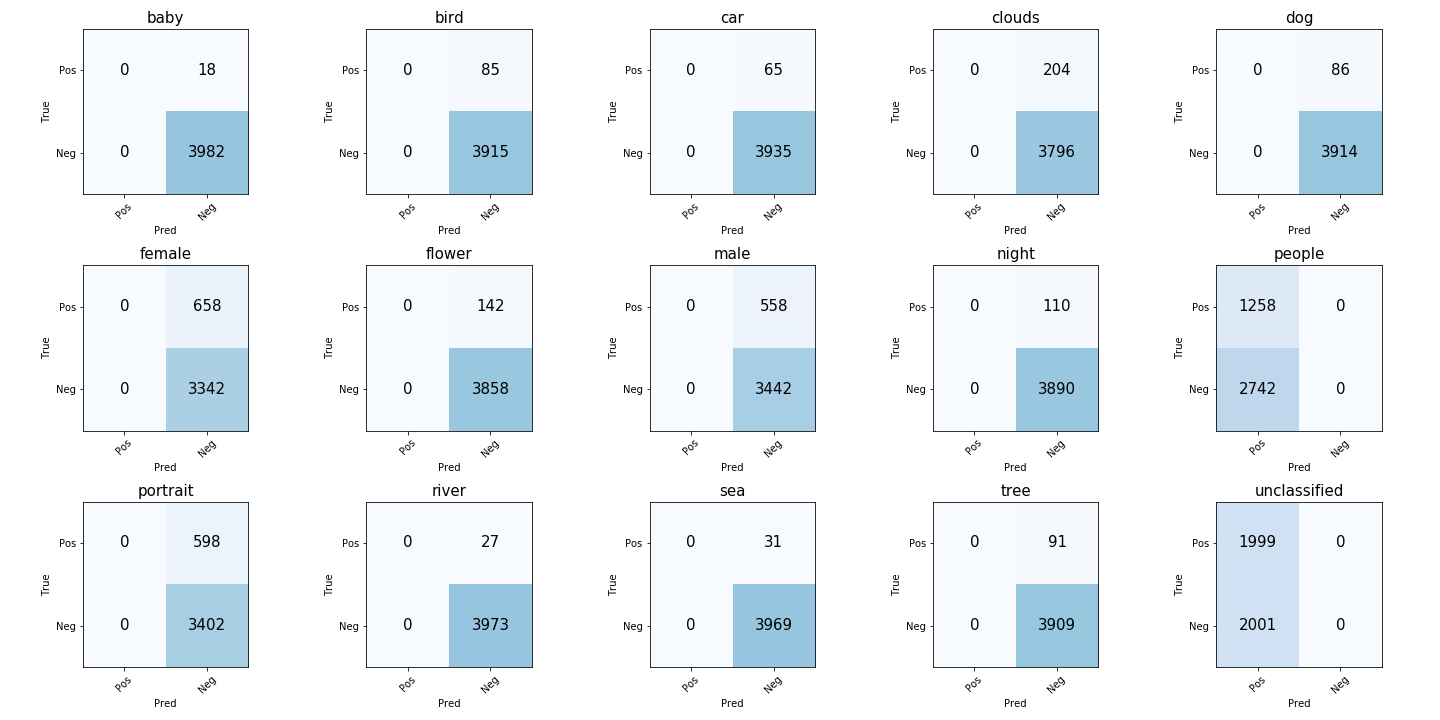
\includegraphics[width=\textwidth]{images/final_model_confusion.png}
	\begin{itemize}
		\item Always predicts same result for each label on every picture
	\end{itemize}
\end{frame}

\begin{frame}
	\frametitle{\overtitle}
	%\framesubtitle{something}
	\begin{figure}
		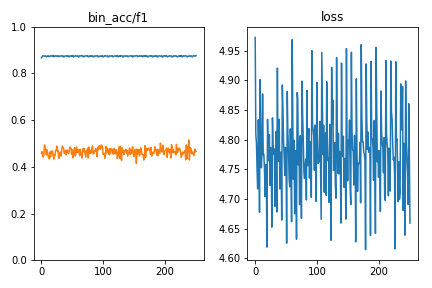
\includegraphics[width=\textwidth]{images/final_model.png}
		\caption{Soemthing}
	\end{figure}
\end{frame}
